After the stock prices were differenced, stabilized, normalized and autoregressively modeled, characteristics of the resulting time series will be examined. While there are easy to apply methods for establishing stationarity and removing trends, some characteristics like structural breaks are most likely hard to remove. Therefore, in some cases not all preconditions are ensured. But the data is not further transformed to enforce less outliers, removed periodicity or ensure ergodicity. By applying yet another transformation in order to achieve those conditions, the data might be polluted in a too drastic way. However, one should be aware of the level of violations for assumptions which are required in correlation analysis.

\begin{figure}
    \centering
    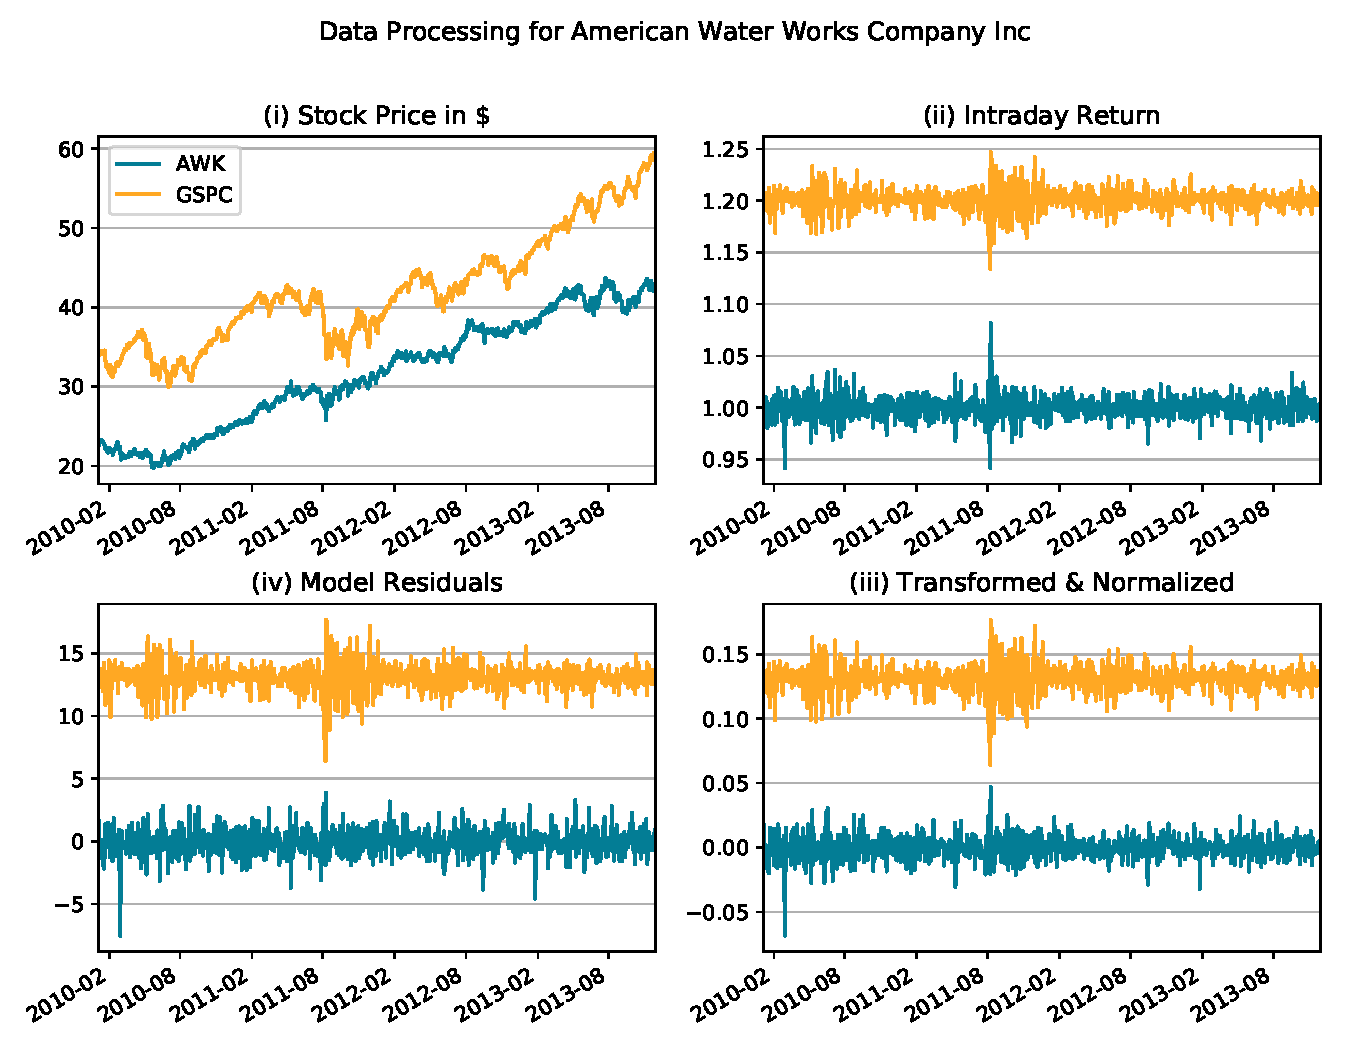
\includegraphics[width=0.9\textwidth]{figures/regression/data-processing-awk.pdf}
    \captionsetup{singlelinecheck=off}
    \caption[foo bar]{Values from intermediate preprocessing steps for the company \emph{American Water Works Company Inc} are shown in blue and compared with the price or intraday return of the S\&P~500 market index in orange. In all cases, the index was scaled and shifted in order to show both time series next to each other. The preprocessing steps are arranged clockwise, starting from the top left corner: \begin{enumerate*}[label=(\roman*)]
        \item unmodified stock prices,
        \item intraday returns,
        \item stabilized and industry-wise normalized returns and
        \item standardized residuals of ARMA(2, 1) and GARCH(1, 1) models on returns.
    \end{enumerate*}}
    \label{fig:data-processing-steps}
\end{figure}

Figure~\ref{fig:data-processing-steps} visualizes the impact of preprocessing on a stock price and takes the S\&P~500 market index into account. In the first plot both time series move strongly similar. After taking the intraday returns, stationarity appears to be ensured but both time series still tend to reveal similarity, e.g. by simultaneous bursts or change in volatility. Subsequently, the return values are stabilized with Box-Cox transformation and normalized by the regarding industry mean. Even though some parts still indicate an existing relationship, the time series is located more stable around zero and reveals less outlier. In the last step, the volatility is adjusted by ARMA and GARCH modelling, resulting in a time series which appears to be very similar to a white noise. Since a white noise process is considered to fulfill almost all constraints in order to be i.i.d., the data seems to be promising for further analysis.


\subsubsection{Stationarity}
\label{subsubsection:stationarity}

The stationarity is one of the most important properties one need to examine before conducting further time series analysis. If it is not present, experiments like correlations or ARMA models lead to falsely results. The stationarity is evaluated by applying hypothesis tests for the presence of unit roots on the examined time series. It is recommended to apply multiple hypothesis tests to provide assurance of a correct outcome, so we will execute the following ones:
\begin{enumerate*}[label=(\roman*)]
    \item Augmented Dickey-Fuller (ADF) \cite{Dickey1976IntroductionSeries}
    \item Phillips-Perron (PP) \cite{Phillips1988TestingRegression}
    \item Kwiatkowski–Phillips–Schmidt–Shin (KPSS) \cite{Kwiatkowski1992TestingRoot}
\end{enumerate*}

The first two test the null hypothesis, that a unit root is present. In contrast, the latter one tests the null hypothesis of stationary data. As common practice (e.g. \cite{Bishara2012TestingApproaches}), the significance level $\alpha=0.05$ is defined for the $p$-value in order to sufficiently reject the null hypothesis.

All three tests are executed on all 467 stock prices at each step of their preprocessing stage. Except for 14 cases, all three tests attest the presence of a unit root in the original stock prices. After taking the intraday returns, there is no stock, for which all three tests simultaneously give evidence for a unit root. Only the KPSS test significantly rejects the absence of unit roots for 15 cases. The following preprocessing steps did not change this number by large, so the final time series can be expected to be stationary.

% "Any series that has a trend will tend to be correlated to any other series that has a trend. For this reason, it is preferable to remove trends and seasonal effects before comparing multiple series. This is usually achieved by working with the residuals of a fitted time series model, such as the regression models of Chapter 3" (Introductory Time Series With R, Cowpertwait and Metcalfe )

% "The model should only be applied to a prewhitened residual series {e_t} that is uncorrelated and contains no trends or seasonal changes, such as might be obtained after fitting a satisfactory SARIMA model." (Cowpertwait and Metcalfe, Page 148, Introductory Time Series with R, 2009)

% RESOLVE unit root: If it cannot be rejected one may run the same test after applying a difference operator like AR(1), AR(2) or Link relatives.
% Diagnostic checking on residuals for:
%   A) Normality 
%   B) Autocorrelation 
%   C) Het.Sce. 
%   D) Test for structural breaks?
%   E) Other properties like periodicity, seasonality and outliers

% Even though there are a lot of factors influencing the stock markets behaviour one needs to cut it down to a few more important variables. Omitting influencing exogeneous factors might lead to spurious correlations / endogeneity but we need to reduce the dimensions of freedom avoiding curse of dimensionality (what is endogeneity: https://www.statisticshowto.datasciencecentral.com/endogenous-variable/) -> Check for endogeneity (error term correlates with independent variable within the model). This would mean that the model is biased and regression analysis using OLS is erroneous. Possible reasons for endogeneity: ommited variables; Measurement error in variable (noise is considered to be part of variable) -> OLS estimation will be biased downwards; Simultaneity (fixed by Instrumental Variables Regression)

% UNIT ROOT: Is it unit root? (explained in background) Apply ADF, PP and/or KPSS as \cite{Vlastakis2012}. Differentiate between trend-stationary, difference-stationary and just non-stationary. If and only if the null hypothesis of unit root can be rejected, one can apply autoregression; "A finding of a unit root implies that stock returns cannot be predicted." \cite{Narayan2005}. Unit root processes are tíme-series which do not fully recover from shocks. The term originates from a coefficient equal to one for the last value when the next value is calculated, hiding/covering the underlying trend ones is looking for.


\subsubsection{Data Distribution}
\label{subsubsection:normal_dist}

% Many financial variables are non-normally distributed (Mandelbrot and Benuit 1963)

Another precondition of cross-correlation are normal distributed samples \cite{Bishara2012TestingApproaches}. For evaluating if the data distribution is similar to a normal distribution, again hypothesis tests are a good way to acquire evidence in favour of or against normality being present. For example, \citet{Vlastakis2012InformationVolatility} use the Jarque-Bera test \cite{Jarque1980EfficientResiduals} to inspect the null hypothesis that a normal distribution is present. Conducted on the 30 stocks from Dow Jones Industrial Average, they reject the presence of a normal distribution with 99~\% confidence. As stated in the previous section, it is a common practice to use multiple tests for double-checking the results. For this task, the following are applied which all rely on the same null hypothesis of normality being present:
\begin{enumerate*}[label=(\roman*)]
    \item Jarque-Bera (JB) \cite{Jarque1980EfficientResiduals}
    \item Shapiro-Wilk (SW) \cite{Shapiro1965AnSamples}
    \item D’Agostino’s K\^2 (DK2) \cite{DAgostino1973Testsb}
    \item Anderson-Darling (AD) \cite{Stephens1974EDFComparisons}
\end{enumerate*}

As might be expected from the initial analysis of kurtosis and skewness in Section~\ref{subsubsection:processing:stationarity}, only 16 out of 467 preprocessed stock prices reveal evidence for a normal distribution by at least one test statistic.


To inspect the possibility of another distribution, the Kolmogorow-Smirnow (KS) \cite{Massey1951TheFit} test is applied. It assesses the equality of two distributions by calculating the distance of their cumulative distribution function. The distributions of each preprocessed stock prices is compared to a set of common probability distributions. The most frequently distribution (using a rejection rate of $\alpha=0.05~\%$) was Student's $t$ with 7 dimensions of freedom in average, followed by logistic, laplace and normal distribution. Based on the suggested distributions, the data appears to have heavier tails as a normal distribution. % Still, the normal distribution appears to be a reasonable assumption for 304 out of 467 preprocessed stock return series and the close average kurtosis and skewness provide evidence for the suitability. Except for the examination of outliers, the data will therefore be treated as a normal distribution.

These findings do not lead to the conclusion that calculating the correlation on such non-normal data returns erroneous conclusion. The Pearson correlation coefficient, which will be introduced later, is fairly robust for different data distributions, although it does assume normality. Only if the distribution differs strongly from normality, e.g. by extreme values for skew or kurtosis, it should be treated with caution \cite{Bishara2012TestingApproaches}.

% https://sci-hub.se/10.2466/pms.1976.43.3f.1319


\subsubsection{Homoscedasticity}
\label{subsubsection:homoscedasticity}

Economic variables like stock prices are known to potentially exhibit heteroscedasticity \cite{Salisu2016UnitSeries}. To examine linear versions of heteroscedasticity, the Breusch-Pagan test (BP) \cite{Breusch1979AVariation} can be used. If this test fails to reject the null hypothesis of homoscedasticity and therefore indicates the presence of homoscedasticity, the White test \cite{White1980AHeteroskedasticity} can be applied to test for nonlinear forms. It checks the null hypothesis on a greater set of terms which needs more calculation and might reveal less significant results than BP. Because of the large number of degrees of freedom, the White test can over-react. Concluding, both tests are applied in the following. % https://www3.nd.edu/~rwilliam/stats2/l25.pdf

While at least one test indicated heteroscedasticity for 422 stocks based on their intraday return values, 307 remained with significant results after transformation and normalization. The enhanced stability in form of volatility, gives subsequent justification for the previous prewhitening steps. In more than a half of these cases the White test revealed sufficient evidence while the BP did not. This leads to the conclusion that in many cases the data contains nonlinear heteroscedasticity, which BP is not able to detect.

After applying the GARCH model, 28 stocks remain which do not satisfy both tests for homoscedasticity. Besides those 28 stocks, 94 stocks have at least one test showing evidence for rejecting the null hypothesis. Most of these show evidence for the White test. Since this leads to the conclusion that there is still nonlinear heteroscedasticity present, the GARCH model might be not the best model and a more sophisticated approach like a nonlinear GARCH might be more suitable in future work. However, a large proportion of heteroscedasticity was removed compared to the original stock returns.

% (White Test with stats.diagnostic.het_white [from https://machinelearningmastery.com/develop-arch-and-garch-models-for-time-series-forecasting-in-python/)], BP test including the squared value, Engle's ARCH test (null=homo), Levene's Test -> https://sci-hub.se/10.2307/2328672) 

% (https://www.researchgate.net/post/How_to_remove_serial_correlation_and_heteroskedasticity) (https://mpra.ub.uni-muenchen.de/54954/1/MPRA_paper_54954.pdf) (https://sci-hub.se/10.1080/00036840802600087)

\subsubsection{Structural Breaks}
\label{subsubsection:structural_breaks}

% Additionally, the following analysis inspects the time series on structural breaks like shifts or bursts, and heteroscedasticity (heterogeneous volatility) \cite{xxxSalisu2016}.

Regression models, which are broadly used for hypothesis testing and other purposes, are established by estimating the coefficient of regressors fitting the dependent variable. A big issue of such coefficients are their stability. If the regressed variables contain structural changes like a level shift in mean or volatility, the estimated coefficients are most likely to be not suitable. If a specific point of time should be examined regarding a structural break, tests can be used which compare the regression coefficients which are calculated separately on each half of the dataset. If the coefficients are sufficiently different from each other, the time series can be assumed to have a structural break at the chosen time stamp.

However, examining the existence of structural breaks in an unsupervised manner, i.e. at an unknown point of time, appears to be a more difficult topic. Even, the application of machine learning for unsupervised anomaly detection is an ongoing topic, which is not completely reliable. All the more, the automated check using a statistical approach should be viewed skeptical. Therefore, only evidence for the presence of an unknown number of structural breaks is collected. The work will not further deal with it, accepting their presence for a few cases. The CUSUM-test \cite{Brown1975TechniquesTime} can be used for these cases, testing the null hypothesis of stable coefficients of a linear regression model.

Only two out of all original stock prices are assumed to contain at least one structural break following the CUSUM-test. The number increases only slightly after differencing and normalization concluding with 22 stocks revealing unstable coefficients. Even though, we are trying to remove the mean movement across one industry, not all prices might contain this common behaviour for the entire period. For some stock prices, the normalization step appears to introduce a new movement sectionally which leads to the significant rejection of stable coefficients over the entire times series.

\subsubsection{Autocorrelation}
\label{subsubsection:autocorrelation}

To test the autocorrelation across the whole dataset, two hypothesis tests were applied. The Durbin-Watson statistic \cite{Durbin1971TestingRegression.III} returns a number between 0 and 4 with suggesting no autocorrelation for the first lag if the statistic falls between 1.5 and 2.5. The Ljung-Box Q Test \cite{Dionisio2004MutualSeries} was also applied on the first lag only and tests the null hypothesis of no autocorrelation. Before applying autoregressive models, the preprocessing already reduced the number of first-lag autocorrelated stock returns from 467 down to 82 which was also observed previously by looking at the significant lags of ACF and PACF in Section~\ref{subsubsection:processing:ar_modelling}. For these remaining cases, the modelling was applied and successfully cleared the autocorrelation completely for all time series.

\subsubsection{Further Properties}

Variables and their regarding distributions are hard to describe without visualizing the data. descriptive properties like skewness, kurtosis and heteroscedasticity are provided, but they can not fully reflect the data itself. Even though stationarity is validated, latent periodic patterns can still remain.

\paragraph{Seasonality} 
Following the decomposition model, some autoregressive patterns can be describes by seasonality (recurring at fixed time intervals) or cyclicality (recurring patterns without fixed time frames). Since the data preprocessing does not account for these properties, it needs to be conducted if there is evidence for such periodic patterns. Especially, daily prices are prone to seasonality in form of weekly, monthly or seasonal patterns. Since two stock prices might follow the same pattern, there is always a chance of falsely correlating stock prices. Related work suggests using a differencing window over a year, so only two days from the same time of a year are always compared. Despite of a sliding window, this would decrease the number of resulting data points by about 250 samples (number of trading days in one year) which is critical for the size of the dataset used in this work.

% Seasonality can be fixed by increasing the differencing window (e.g. diff over a year to fix months). Microscopic patterns (e.g. on a weekly basis) are hard to detect.  Finding sporadic occurring patterns, seasonality or periodicity in noisy data like stock prices is a difficult topic, missing a panacea for the correct method. Even though, those characteristics should be considered in regression analysis, you never can be sure to have them removed and work on clean un-autocorrelated data. e.g. for expected seasonality: December Effect (https://www.timothysykes.com/blog/seasonal-stocks/)

\begin{figure}[!ht]
    \centering
    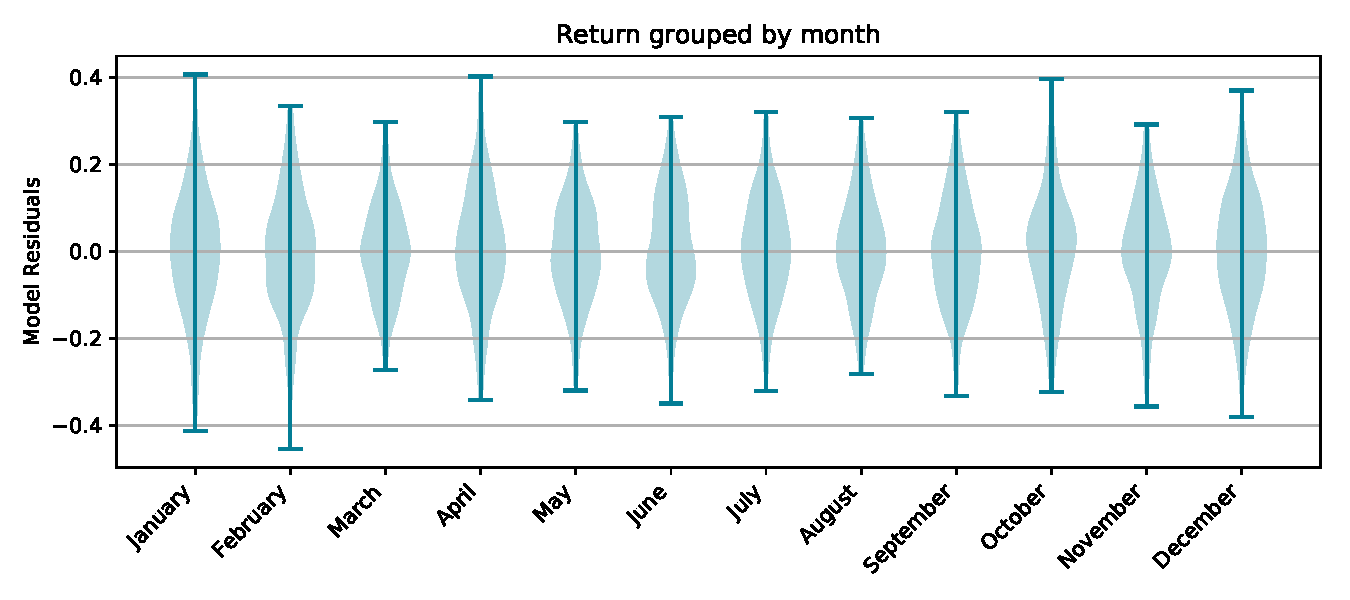
\includegraphics[width=\textwidth]{figures/regression/returns-per-month.pdf}
    \caption{Violin plot of preprocessed return values, denoted as model residuals, after taking the mean for each month and stock. The filled area visualizes the approximated data distribution along the vertical line}
    \label{fig:boxplot_seasons}
\end{figure}

Figure~\ref{fig:boxplot_seasons} shows the averaged model residuals for each month and stock. For every month the mean is not significantly different from zero but the standard deviation partially varies across the year. The lowest standard deviation is observed for the 467 values in March which equals 0.0998. The highest standard deviation 0.1266 is observed for January indicating a slightly increased uncertainty after the Christmas business. However, these result shows that there is no observable seasonality measured upon the mean monthly values. The same analysis was conducted for separate industries, too. While there is a significant seasonality visible on the original returns, they disappear after normalizing by the industry-wide mean, leading to similar zero-mean distribution as in Figure~\ref{fig:boxplot_seasons}.


\paragraph{Outliers}
Outliers are usually described as unexpected data points with an abnormal distance from the center of the data. The removal of such outliers is common but questionable practice since it can affect data properties. Unfortunately, there it is not easy to determine outliers in a non-parametric fashion for an arbitrary data distribution. A Student's $t$-distribution is most likely to fit the acquired data as pointed out before. Similar to the interquartile method for a normal distribution, an observation is seen as an outlier if it exceeds a chosen confidence interval. Suitable values for the distribution parameters (dimension of freedom, location and scale) are determined for each stock separately. Based on these parameters, the 99.5~\% confidence interval is calculated. Per definition, only 0.5~\%, i.e. five out of 984 observations, ought to be outside of this interval. On the preprocessed data, 199 stocks contain more than five outliers, but no more than seven.

\begin{figure}[!ht]
    \centering
    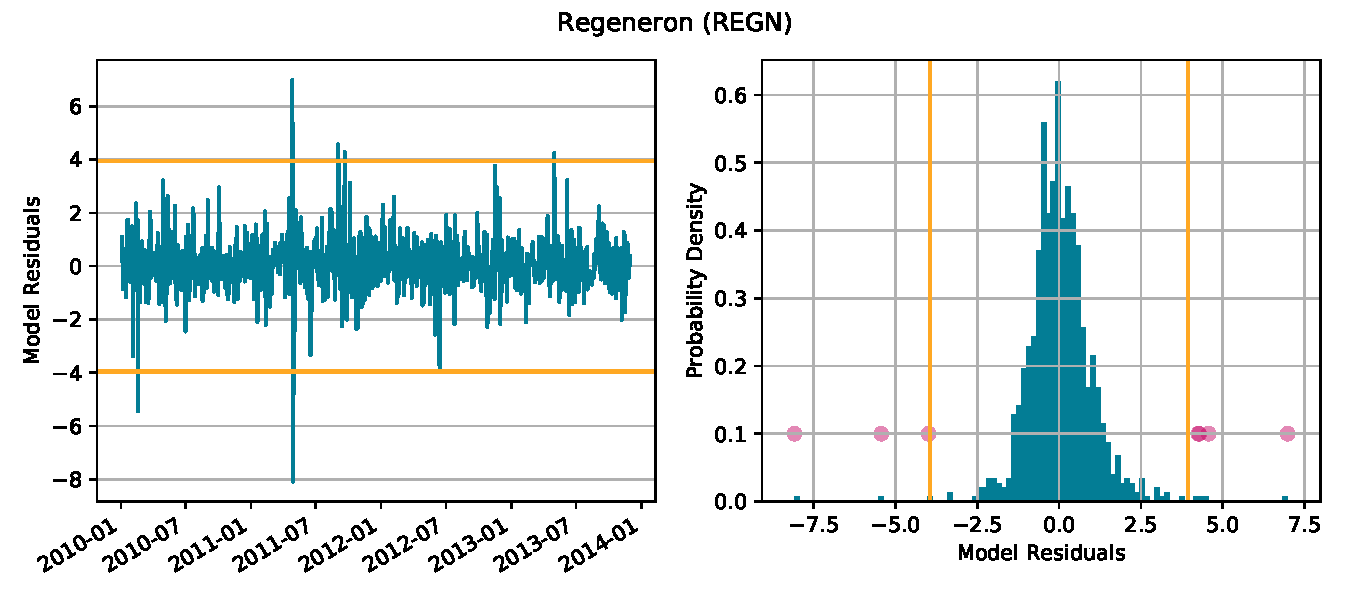
\includegraphics[width=\textwidth]{figures/regression/data-outliers-REGN.pdf}
    \caption{Preprocessed stock return and density histogram of those values for company \emph{Regeneron}. The orange line denotes the 99.5~\% confidence interval for a Student's $t$ distribution with four dimensions of freedom. On seven days an extreme value was observed which is denoted by a purple circle in the histogram on the right. The greatest two outliers can be observed for the 27th of April, 2011.}
    \label{fig:data_outliers}
\end{figure}

One stock with seven outliers is shown in Figure~\ref{fig:data_outliers}. At the 27th of April in 2011, the stock underwent a fast increase and decrease in value. This anomalous behaviour was caused by a successful study regarding a new drug for treatment of advanced colorectal cancer. The article \emph{\enquote{Regeneron, Sanofi Therapy Extends Lives of Colorectal Cancer Patients}} by Bloomberg, published in the evening of the 26th of April, reported these results.
 
Because removal or scaling down of unexpected extreme values, transforms the data in an unreasonable fashion and because it is not feasible to determine which data point should be considered actually unexpected, the outliers will not be treated different from the other data points. However, it is still worth mentioning that the number of outliers is not far above the expected value and therefore considered to not raise a sufficient influence on the data analysis.

% On the basis of a normal distribution, an observation would be to assumed to be an outlier if it falls below $Q1-1.5\times IQR$ or above $Q3+1.5\times IQR$, where $Q1$ and $Q3$ refer to the first and third quartile and $IQR$ to the interquartile range of the data.

% On the residuals, again the full analysis of characteristics was executed. In terms of stationarity, data distribution, heteroscedasticity, structural breaks and outliers no substantial change was observed.